\documentclass[12pt]{article}
\usepackage[english]{babel}
\usepackage[utf8]{inputenc}

%% Pointer to 'default' preamble
% pacakages and definitions

\usepackage{geometry}
\geometry{
	letterpaper, 
	portrait, 
	top=.75in,
	left=.8in,
	right=.75in,
	bottom=.5in		} 	% Page Margins
	
%% additional packages for nice things
\usepackage{amsmath} 	% for most math
\usepackage{commath} 	% for abs
\usepackage{lastpage}	% for page count
\usepackage{amssymb} 	% for therefore
\usepackage{graphicx} 	% for image handling
\usepackage{wrapfig} 	% wrap figures
\usepackage[none]{hyphenat} % for no hyphenations
\usepackage{array} 		% for >{} column characterisctis
\usepackage{physics} 	% for easier derivative \dv....
\usepackage{tikz} 		% for graphic@!
\usepackage{circuitikz} % for circuits!
\usetikzlibrary{arrows.meta} % for loads
\usepackage[thicklines]{cancel}	% for cancels
\usepackage{xcolor}		% for color cancels
\usepackage[per-mode=fraction]{siunitx} % for si units and num
\sisetup{group-separator = {,}, group-minimum-digits = 3} % additional si unit table functionality

\usepackage{fancyhdr} 	% for header
\usepackage{comment}	% for ability to comment out large sections
\usepackage{multicol}	% for multiple columns using multicols
\usepackage[framed,numbered]{matlab-prettifier} % matlab sytle listing
\usepackage{marvosym} 	% for boltsymbol lightning
\usepackage{pdflscape} 	% for various landscape pages in portrait docs.
%\usepackage{float}
\usepackage{fancyvrb}	% for Verbatim (a tab respecting verbatim)
\usepackage{enumitem}	% for [resume] functionality of enumerate
\usepackage{spreadtab} 	% for using formulas in tables}
\usepackage{numprint}	% for number format in spread tab
\usepackage{subcaption} % for subfigures with captions
\usepackage[normalem]{ulem} % for strike through sout

% for row colors in tables....
\usepackage{color, colortbl}
\definecolor{G1}{gray}{0.9}
\definecolor{G2}{rgb}{1,0.88,1}%{gray}{0.6}
\definecolor{G3}{rgb}{0.88,1,1}

% For table formatting
\usepackage{booktabs}
\renewcommand{\arraystretch}{1.2}
\usepackage{floatrow}
\floatsetup[table]{capposition=top} % put table captions on top of tables

% Caption formating footnotesize ~ 10 pt in a 12 pt document
\usepackage[font={small}]{caption}

%% package config 
\sisetup{output-exponent-marker=\ensuremath{\mathrm{E}}} % for engineer E
\renewcommand{\CancelColor}{\color{red}}	% for color cancels
\lstset{aboveskip=2pt,belowskip=2pt} % for more compact table
%\arraycolsep=1.4pt\def
\setlength{\parindent}{0cm} % Remove indentation from paragraphs
\setlength{\columnsep}{0.5cm}
\lstset{
	style      = Matlab-editor,
	basicstyle = \ttfamily\footnotesize, % if you want to use Courier - not really used?
}
\renewcommand*{\pd}[3][]{\ensuremath{\dfrac{\partial^{#1} #2}{\partial #3}}} % for larger pd fracs
\renewcommand{\real}[1]{\mathbb{R}\left\{ #1 \right\}}	% for REAL symbol
\newcommand{\imag}[1]{\mathbb{I}\left\{ #1 \right\}}	% for IMAG symbol
\definecolor{m}{rgb}{1,0,1}	% for MATLAB matching magenta
	
%% custom macros
\newcommand\numberthis{\addtocounter{equation}{1}\tag{\theequation}} % for simple \numberthis command

\newcommand{\equal}{=} % so circuitikz can have an = in the labels
\newcolumntype{L}[1]{>{\raggedright\let\newline\\\arraybackslash\hspace{0pt}}m{#1}}
\newcolumntype{C}[1]{>{\centering\let\newline\\\arraybackslash\hspace{0pt}}m{#1}}
\newcolumntype{R}[1]{>{\raggedleft\let\newline\\\arraybackslash\hspace{0pt}}m{#1}}

%% Header
\pagestyle{fancy} % for header stuffs
\fancyhf{}
% spacing
\headheight 29 pt
\headsep 6 pt

%% Header
\rhead{Thad Haines \\ Page \thepage\ of \pageref{LastPage}}
\chead{PST s\_simu\_Batch Flow Chart\\ }
\lhead{Research \\ 6/9/20}

%% Flow chart specific packages
\usepackage{tikz}
%\usepackage{amsmath}
%\usepackage{comment}
\usetikzlibrary{shapes.geometric, arrows, positioning}
\usetikzlibrary{calc,shapes,shapes.multipart}
\tikzstyle{arrow} = [thick,->,>=stealth]


%% Flow chart custom shapes
% Terminal
\tikzstyle{terminal} = [rectangle, rounded corners, minimum width=3cm, minimum height=1cm,text centered, text width=3cm, draw=black]

% Process
\tikzstyle{process} = [rectangle, minimum width=3cm, minimum height=1cm, text centered,text width=4cm, draw=black]

% Decision
\tikzstyle{decision} = [diamond, aspect=1.8, minimum width=2cm, minimum height=1cm, text centered, text width=2cm, draw=black]

% Subprocess
\newcommand\ppbb{path picture bounding box}
\tikzset{
	subprocess/.style = {rectangle, draw=black, 
		minimum width=4.3cm, minimum height=1cm, inner xsep=3mm,
		text width =\pgfkeysvalueof{/pgf/minimum width}-2*\pgfkeysvalueof{/pgf/inner xsep},
		align=flush center,
		path picture={\draw 
			([xshift =2mm] \ppbb.north west) -- ([xshift= 2mm] \ppbb.south west)
			([xshift=-2mm] \ppbb.north east) -- ([xshift=-2mm] \ppbb.south east);
		},% end of path picture
	}
}

% bubble note
\tikzstyle{note} = [fill, ellipse,fill=gray!20, node distance=4cm, minimum height=1em, text width=3cm, text centered]

%Off page connector
\tikzset{
pageconD/.style={shape=signal,draw, signal to=south,minimum width=3em,text height=1.5em,align=center}
}
\tikzset{
pageconU/.style={shape=signal,draw, signal to=north,minimum width=3em,text height=1.5em,align=center}
}

\begin{document}
% Modified to be multi pages with breaks
%===============================================================================
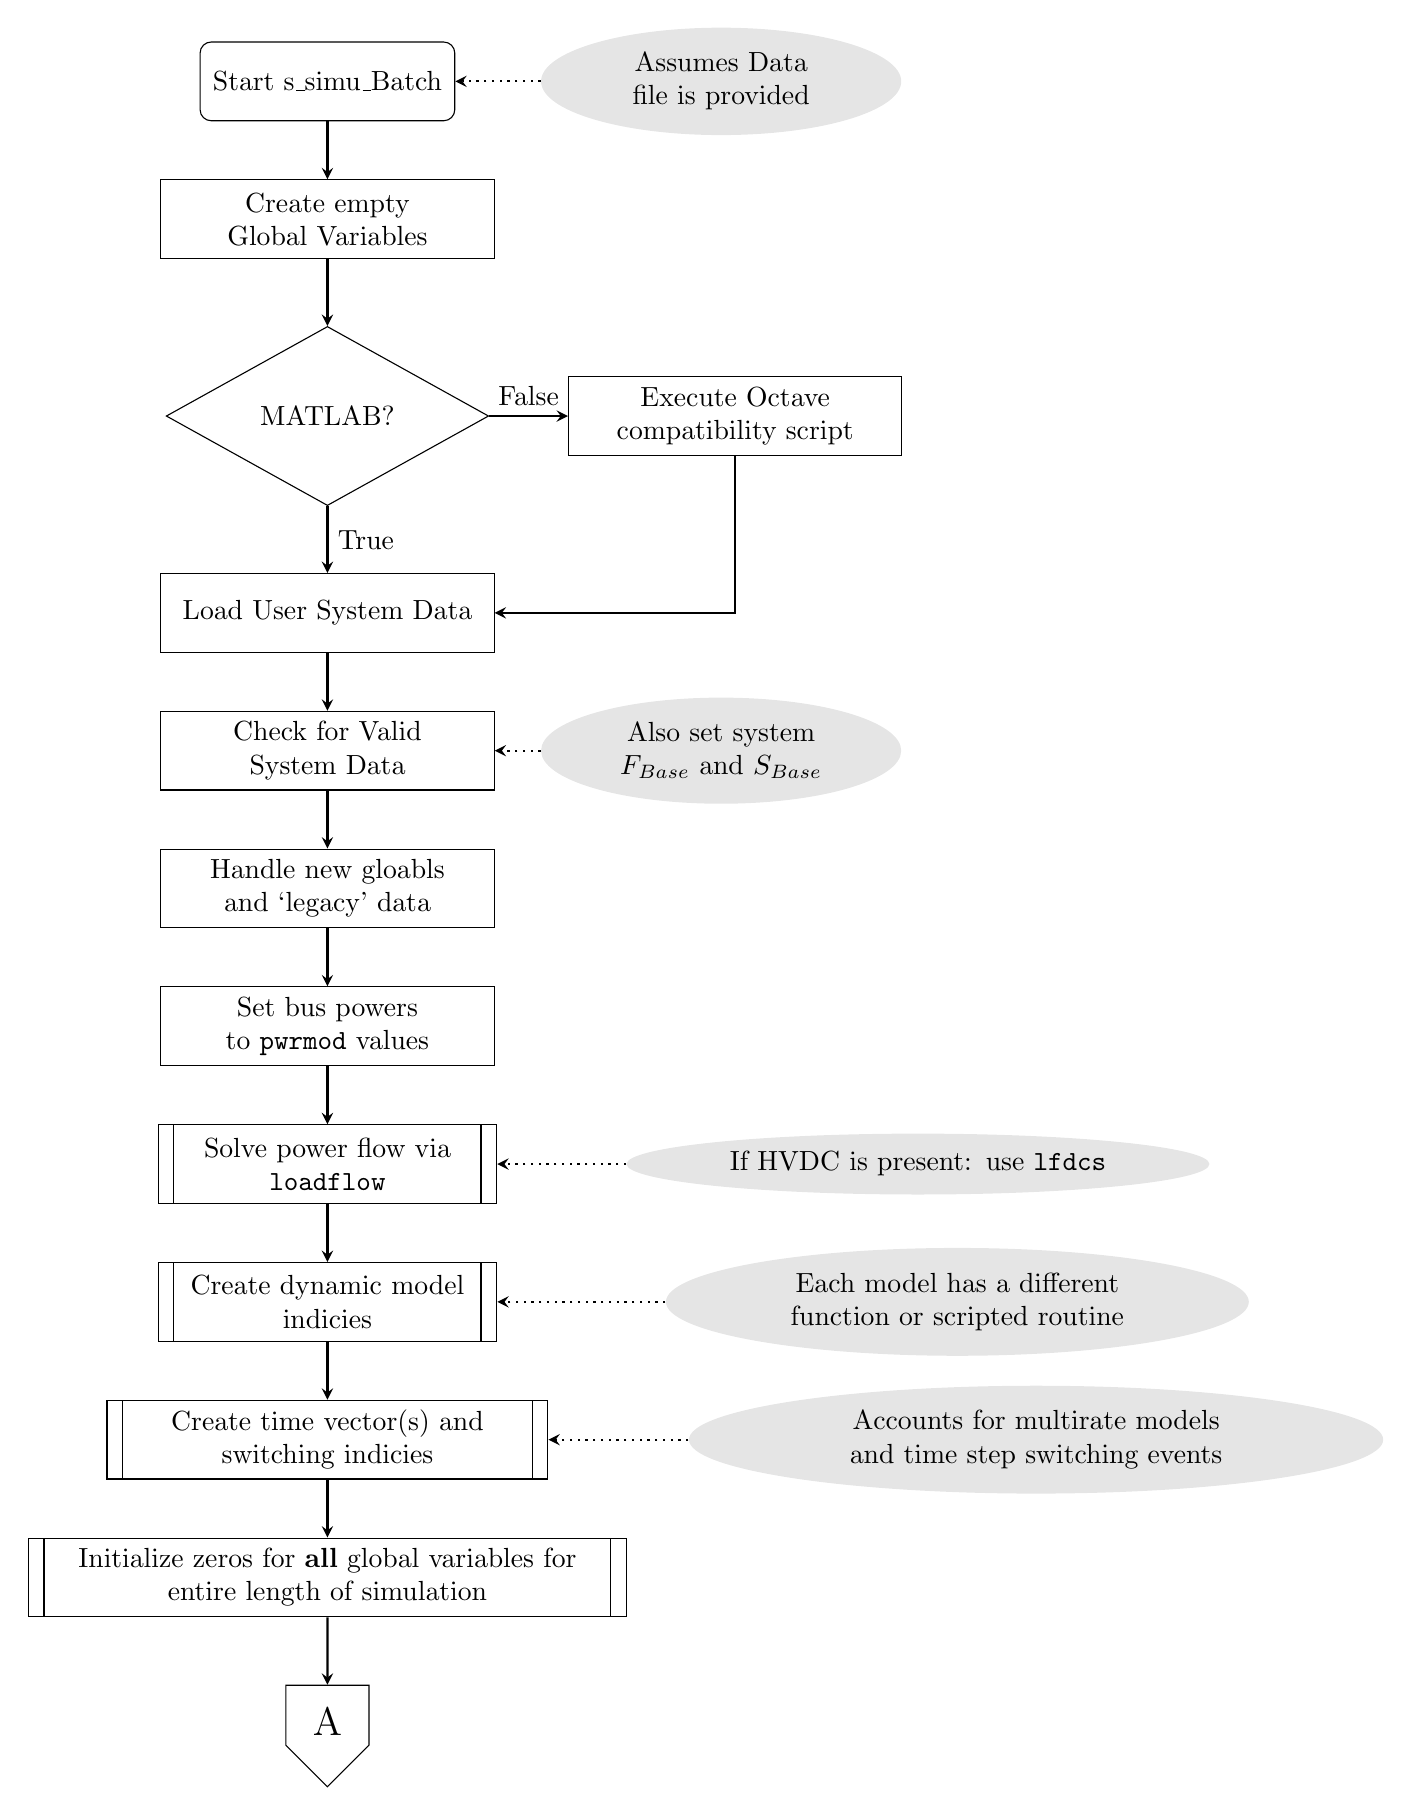
\begin{tikzpicture}[node distance=1.75cm] 
%----------------------------------------------------------------------------
% Placement of flowcart nodes
\node (start) [terminal] {Start s\_simu\_Batch};
\node (createGlobals) [process, below of = start] {Create empty Global Variables};
% matlab decision block
\node (checkProg) [decision, below of=createGlobals, yshift=-.75cm, text width=3cm] {MATLAB?};
\node (octaveComp) [process, right = 1 cm of checkProg] {Execute Octave compatibility script};

\node (loadData) [process, below of = checkProg, yshift=-.75cm] {Load User System Data};
\node (checkUserData) [process, below of = loadData] {Check for Valid System Data};
\node (handleNewGlobals) [process, below of = checkUserData] {Handle new gloabls and `legacy' data};
\node (pwrModInitCheck) [process, below of = handleNewGlobals] {Set bus powers to \verb|pwrmod| values};

\node (initPF) [subprocess, below of = pwrModInitCheck] {Solve power flow via \verb|loadflow|};
\node (createModelIndicies) [subprocess, below of = initPF] {Create dynamic model indicies};
\node (createTimeVectors) [subprocess, below of = createModelIndicies, text width = 5 cm] {Create time vector(s) and switching indicies};
\node (initializeZeros) [subprocess, below of = createTimeVectors, text width = 7 cm] {Initialize zeros for \textbf{all} global variables for entire length of simulation};

\node (page1End) [pageconD, below of = initializeZeros ] {\Large A};

%----------------------------------------------------------------------------
% Draw lines
\draw [arrow] (start) -- (createGlobals);
\draw [arrow] (createGlobals) -- (checkProg);
\draw [arrow] (octaveComp) |- (loadData);

\draw [arrow] (loadData) -- (checkUserData);
\draw [arrow] (checkUserData) -- (handleNewGlobals);
\draw [arrow] (handleNewGlobals) -- (pwrModInitCheck);
\draw [arrow] (pwrModInitCheck) -- (initPF);

\draw [arrow] (initPF) -- (createModelIndicies);
\draw [arrow] (createModelIndicies) -- (createTimeVectors);
\draw [arrow] (createTimeVectors) -- (initializeZeros);
\draw [arrow] (initializeZeros) -- (page1End);

%----------------------------------------------------------------------------
% Draw Decision Lines
\draw [arrow] (checkProg) --  node[anchor=south] {False} (octaveComp);
\draw [arrow] (checkProg) --  node[anchor=west] {True} (loadData);

%----------------------------------------------------------------------------
% Notes and edges
%\node [left of= start, node distance = 7 cm](title){{\Large System Initialization}};

\node [note, right of=start, node distance =5cm](note1){Assumes Data file is provided};
\draw [arrow,dotted] (note1) -- (start);

\node [note, right of=checkUserData, node distance =5cm](note2){Also set system $F_{Base}$ and $S_{Base}$};
\draw [arrow,dotted] (note2) -- (checkUserData);

\node [note, right of=initPF, node distance =7.5cm, text width = 5cm](note3){If HVDC is present: use \verb|lfdcs|};
\draw [arrow,dotted] (note3) -- (initPF);

\node [note, right of=createModelIndicies, node distance =8cm, text width = 5 cm](note4){Each model has a different function or scripted routine};
\draw [arrow,dotted] (note4) -- (createModelIndicies);

\node [note, right of=createTimeVectors, node distance = 9cm,text width=6cm](note5){Accounts for multirate models and time step switching events};
\draw [arrow,dotted] (note5) -- (createTimeVectors);


\end{tikzpicture}
\pagebreak
%===============================================================================


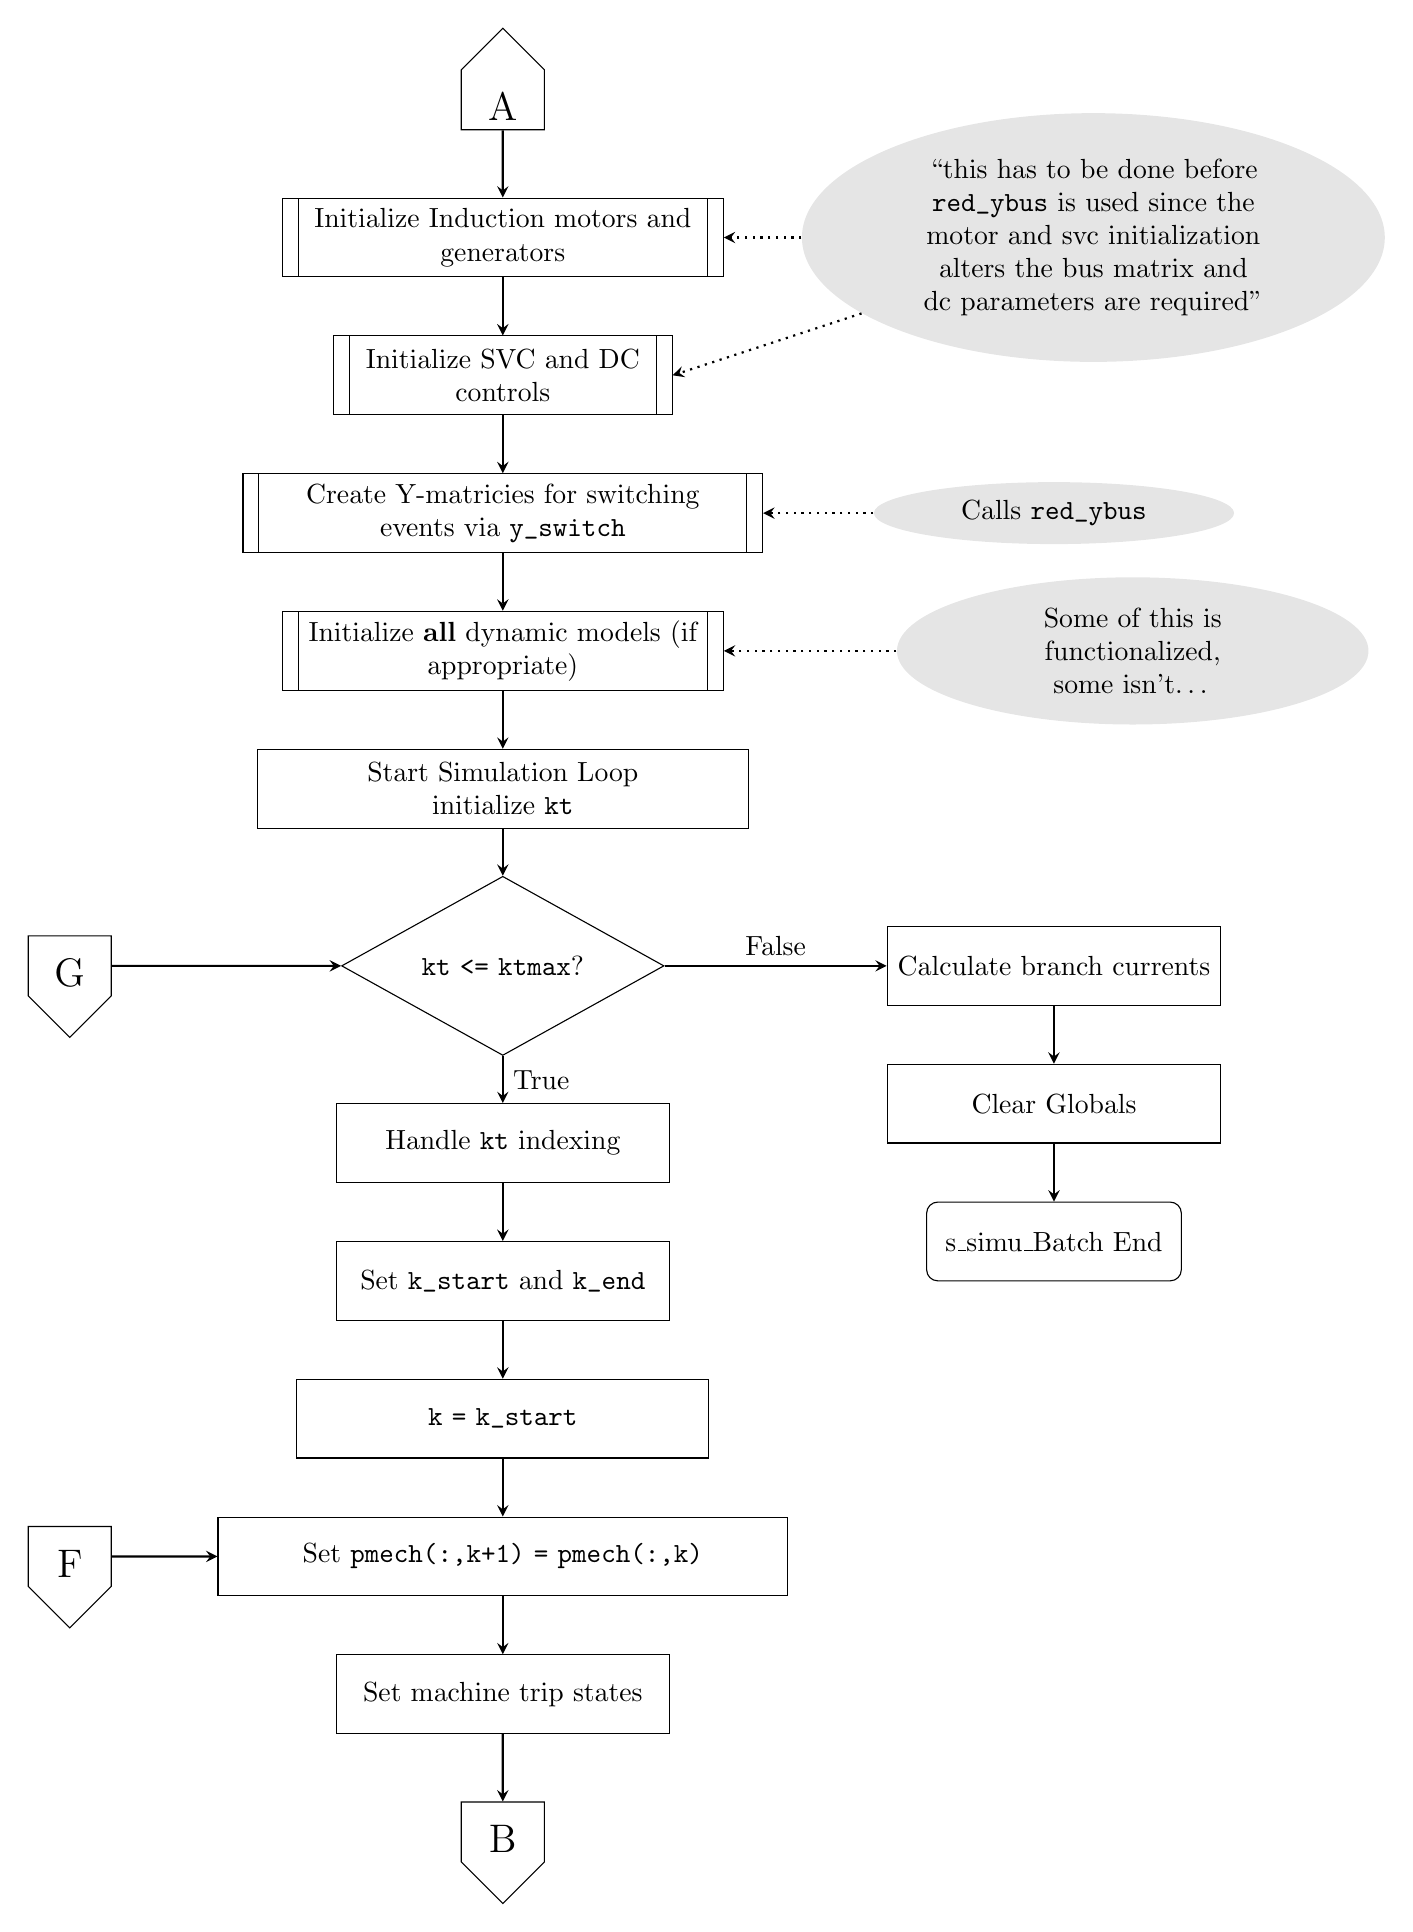
\begin{tikzpicture}[node distance=1.75cm] 
%----------------------------------------------------------------------------
% Placement of flowcart nodes
\node (page2Start) [pageconU ] {\Large A};

\node (initInd) [subprocess, below of = page2Start, text width = 5 cm] 
{Initialize Induction motors and generators};

\node (initSVCandDC) [subprocess, below of = initInd] 
{Initialize SVC and DC controls};

\node (createYswitch) [subprocess, below of = initSVCandDC, text width = 6 cm] 
{Create Y-matricies for switching events via \verb|y_switch|};

\node (initDynamicModels) [subprocess, below of = createYswitch, text width  = 5cm] 
{Initialize \textbf{all} dynamic models (if appropriate)};

\node (startSimLoop) [process, below of = initDynamicModels, text width = 6cm] 
{Start Simulation Loop \\ initialize \verb|kt|};

\node (whileKT) [decision, below of=startSimLoop, yshift=-.5cm, text width=3cm] 
{\verb|kt <= ktmax|?};

\node (KTindex) [process, below of = whileKT, yshift=-.5cm] 
{Handle \verb|kt| indexing};

\node (calcLineI) [process, right of = whileKT, node distance = 7 cm] 
{Calculate branch currents};

\node (cleanGlobals) [process, below of = calcLineI] 
{Clear Globals};

\node (sSimuEnd) [terminal, below of = cleanGlobals] 
{s\_simu\_Batch End};

\node (whileOffPage) [pageconD, left of = whileKT, node distance = 5.5 cm] 
{\Large G};

\node (rangeK) [process, below of = KTindex] 
{Set \verb|k_start| and \verb|k_end|};

\node (forKlength) [process, below of = rangeK, text width = 5cm] 
{\verb|k = k_start|};

\node (setPmech) [process, below of = forKlength, text width = 7cm] 
{Set \verb|pmech(:,k+1) = pmech(:,k)|};

\node (ForOffPage) [pageconD, left of = setPmech, node distance = 5.5 cm]
{\Large F};

\node (tripGen1) [process, below of = setPmech] 
{Set machine trip states};

\node (page2End) [pageconD, below of = tripGen1 ] 
{\Large B};

%----------------------------------------------------------------------------
% Drawing of Lines of main chart
\draw [arrow] (page2Start) -- (initInd);

\draw [arrow] (initInd) -- (initSVCandDC);
\draw [arrow] (initSVCandDC) -- (createYswitch);
\draw [arrow] (createYswitch) -- (initDynamicModels);
\draw [arrow] (initDynamicModels) -- (startSimLoop);

\draw [arrow] (startSimLoop) -- (whileKT);
\draw [arrow] (KTindex) -- (rangeK);
\draw [arrow] (rangeK) -- (forKlength);
\draw [arrow] (forKlength) -- (setPmech);

\draw [arrow] (setPmech) -- (tripGen1);
\draw [arrow] (tripGen1) -- (page2End);

\draw [arrow] (calcLineI) -- (cleanGlobals);
\draw [arrow] (cleanGlobals) -- (sSimuEnd);

% off page connectors
\draw [arrow] (whileOffPage) -- (whileKT);
\draw [arrow] (ForOffPage) -- (setPmech);

%----------------------------------------------------------------------------
%% Note nodes AND edges
\node [note, right of=initInd, node distance = 7.5 cm, text width= 5 cm](note6)
{``this has to be done before \verb|red_ybus| is used since the motor and svc initialization alters the bus matrix and dc parameters are required"};
\draw [arrow,dotted] (note6) -- (initInd);
\draw [arrow,dotted] (note6) -- (initSVCandDC.east);

\node [note, right of=createYswitch, node distance =7cm](note7)
{Calls \verb|red_ybus|};
\draw [arrow,dotted] (note7) -- (createYswitch);

\node [note, right of=initDynamicModels, node distance =8cm, text width = 4cm](note8)
{Some of this is functionalized, some isn't\ldots};
\draw [arrow,dotted] (note8) -- (initDynamicModels);

%----------------------------------------------------------------------------
% Draw Decision Lines
\draw [arrow] (whileKT) --  node[anchor=west] {True} (KTindex);
\draw [arrow] (whileKT) --  node[anchor=south] {False} (calcLineI);
\end{tikzpicture}
\pagebreak
%===============================================================================

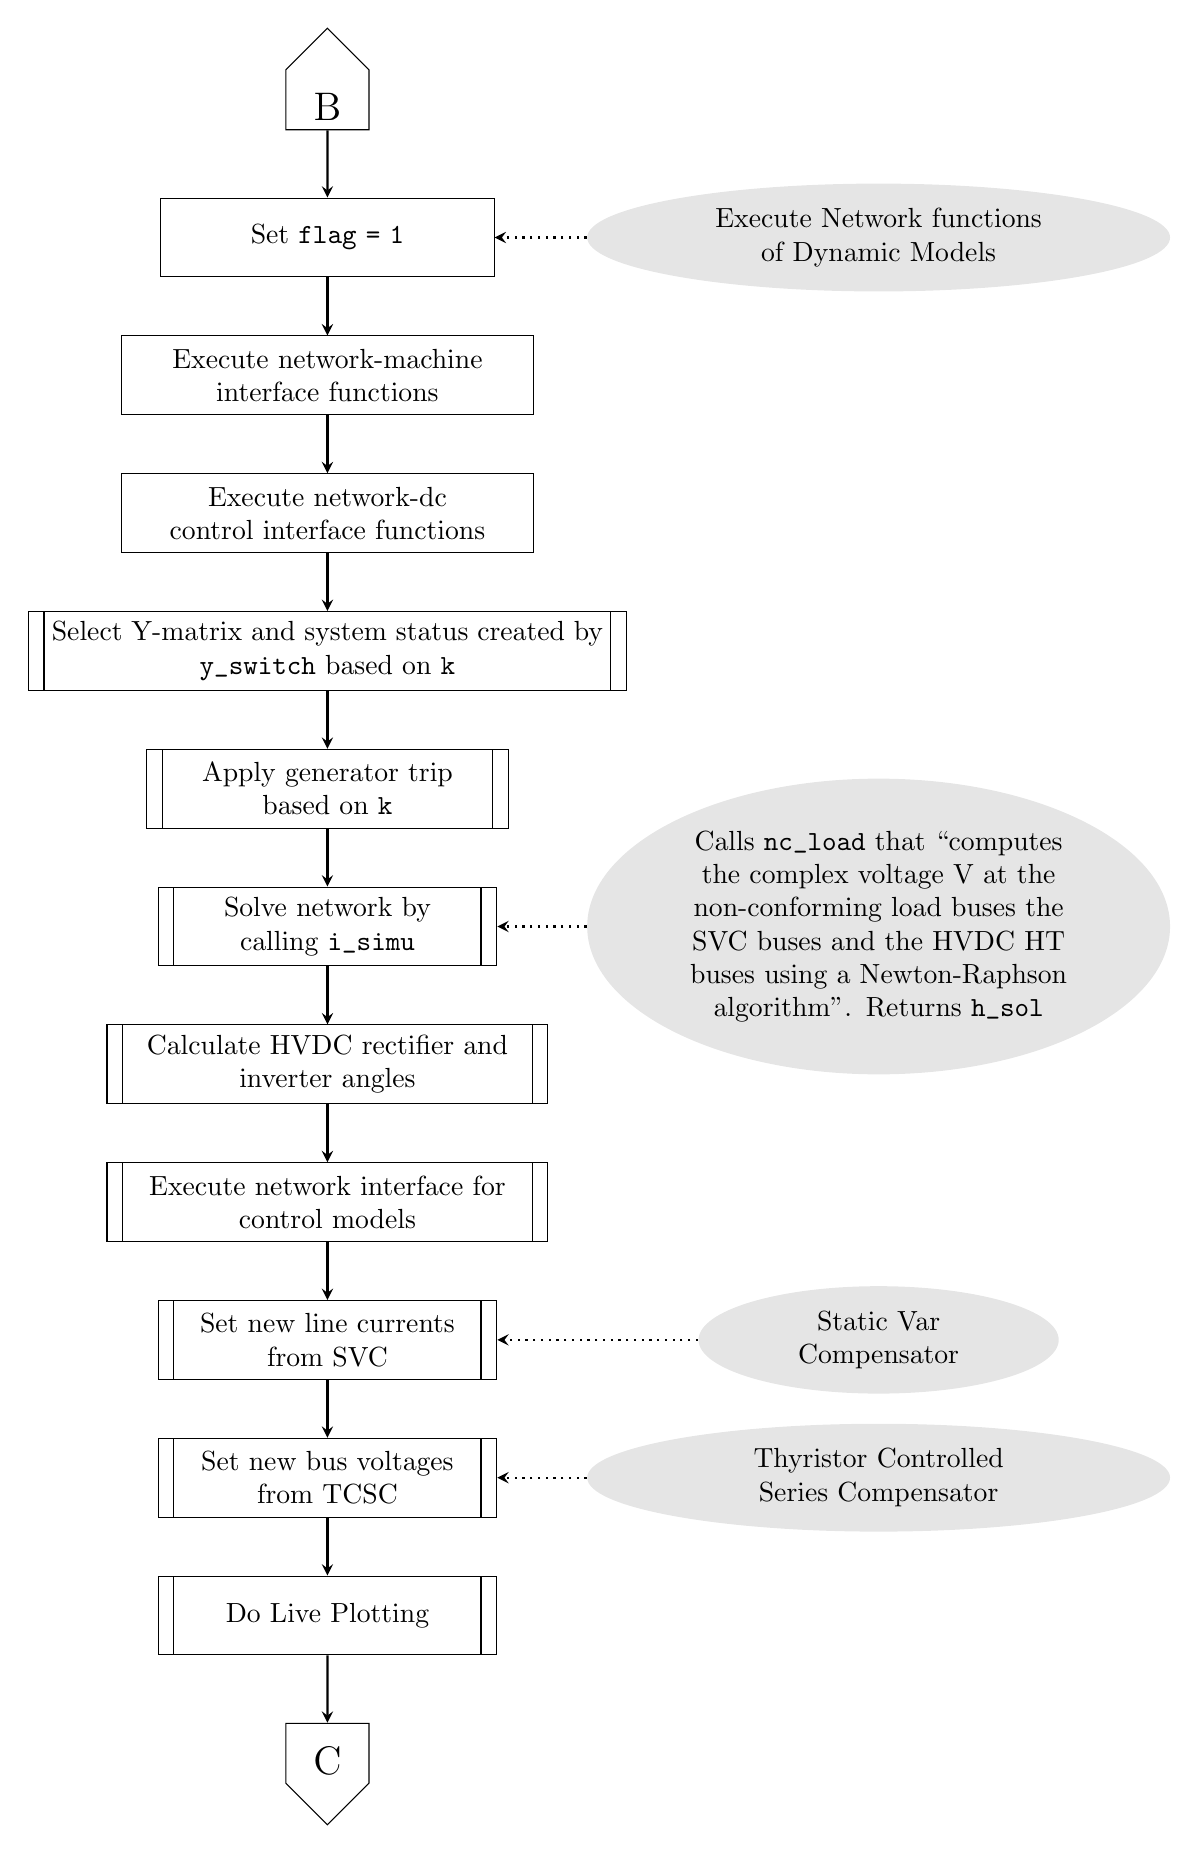
\begin{tikzpicture}[node distance=1.75cm] 
%----------------------------------------------------------------------------
% Placement of flowcart nodes
\node (page3Start) [pageconU ] {\Large B};
\node (setFlagONE1) [process, below of = page3Start] {Set \verb|flag = 1|};
\node (machineInterface1) [process, below of = setFlagONE1, text width = 5cm] {Execute network-machine interface functions};

\node (dcCTRLS1) [process, below of = machineInterface1, text width = 5cm] {Execute network-dc control interface functions};
\node (selectSYS1) [subprocess, below of = dcCTRLS1, text width = 7cm] {Select Y-matrix and system status created by \verb|y_switch| based on \verb|k|};
\node (applyGenTrip) [subprocess, below of = selectSYS1, text width = 4cm] {Apply generator trip based on \verb|k|};
\node (solveNetwork1) [subprocess, below of = applyGenTrip] {Solve network by calling \verb|i_simu|};
%line 1212

\node (HVDC1) [subprocess, below of = solveNetwork1, text width = 5 cm] {Calculate HVDC rectifier and inverter angles};
\node (ctrlNetwork1) [subprocess, below of = HVDC1, text width = 5 cm] {Execute network interface for control models};
\node (Isvc1) [subprocess, below of = ctrlNetwork1] {Set new line currents from SVC};
\node (Vtcsc) [subprocess, below of = Isvc1] {Set new bus voltages from TCSC};

\node (LivePlot) [subprocess, below of = Vtcsc] {Do Live Plotting};
\node (page3End) [pageconD, below of = LivePlot ] 
{\Large C};

%----------------------------------------------------------------------------
% Lines
\draw [arrow] (page3Start) -- (setFlagONE1);
\draw [arrow] (setFlagONE1) -- (machineInterface1);
\draw [arrow] (machineInterface1) -- (dcCTRLS1);

\draw [arrow] (dcCTRLS1) -- (selectSYS1);
\draw [arrow] (selectSYS1) -- (applyGenTrip);
\draw [arrow] (applyGenTrip) -- (solveNetwork1);
\draw [arrow] (solveNetwork1) -- (HVDC1);

\draw [arrow] (HVDC1) -- (ctrlNetwork1);
\draw [arrow] (ctrlNetwork1) -- (Isvc1);
\draw [arrow] (Isvc1) -- (Vtcsc);
\draw [arrow] (Vtcsc) -- (LivePlot);

\draw [arrow] (LivePlot) -- (page3End);

%----------------------------------------------------------------------------
% Notes
\node [note, right of=setFlagONE1, node distance =7cm, text width = 5cm](note2){Execute Network functions of Dynamic Models};
\draw [arrow,dotted] (note2) -- (setFlagONE1);

\node [note, right of=solveNetwork1, node distance =7cm, text width = 5cm](note3){Calls \verb|nc_load| that ``computes the complex voltage V at the non-conforming load buses
the SVC buses and the HVDC HT buses using a Newton-Raphson algorithm". Returns \verb|h_sol|};
\draw [arrow,dotted] (note3) -- (solveNetwork1);

\node [note, right of=Isvc1, node distance =7cm, ](note4){Static Var Compensator};
\draw [arrow,dotted] (note4) -- (Isvc1);

\node [note, right of=Vtcsc, node distance =7cm, text width = 5 cm ](note5){Thyristor Controlled Series Compensator};
\draw [arrow,dotted] (note5) -- (Vtcsc);

\end{tikzpicture}
\pagebreak
%===============================================================================

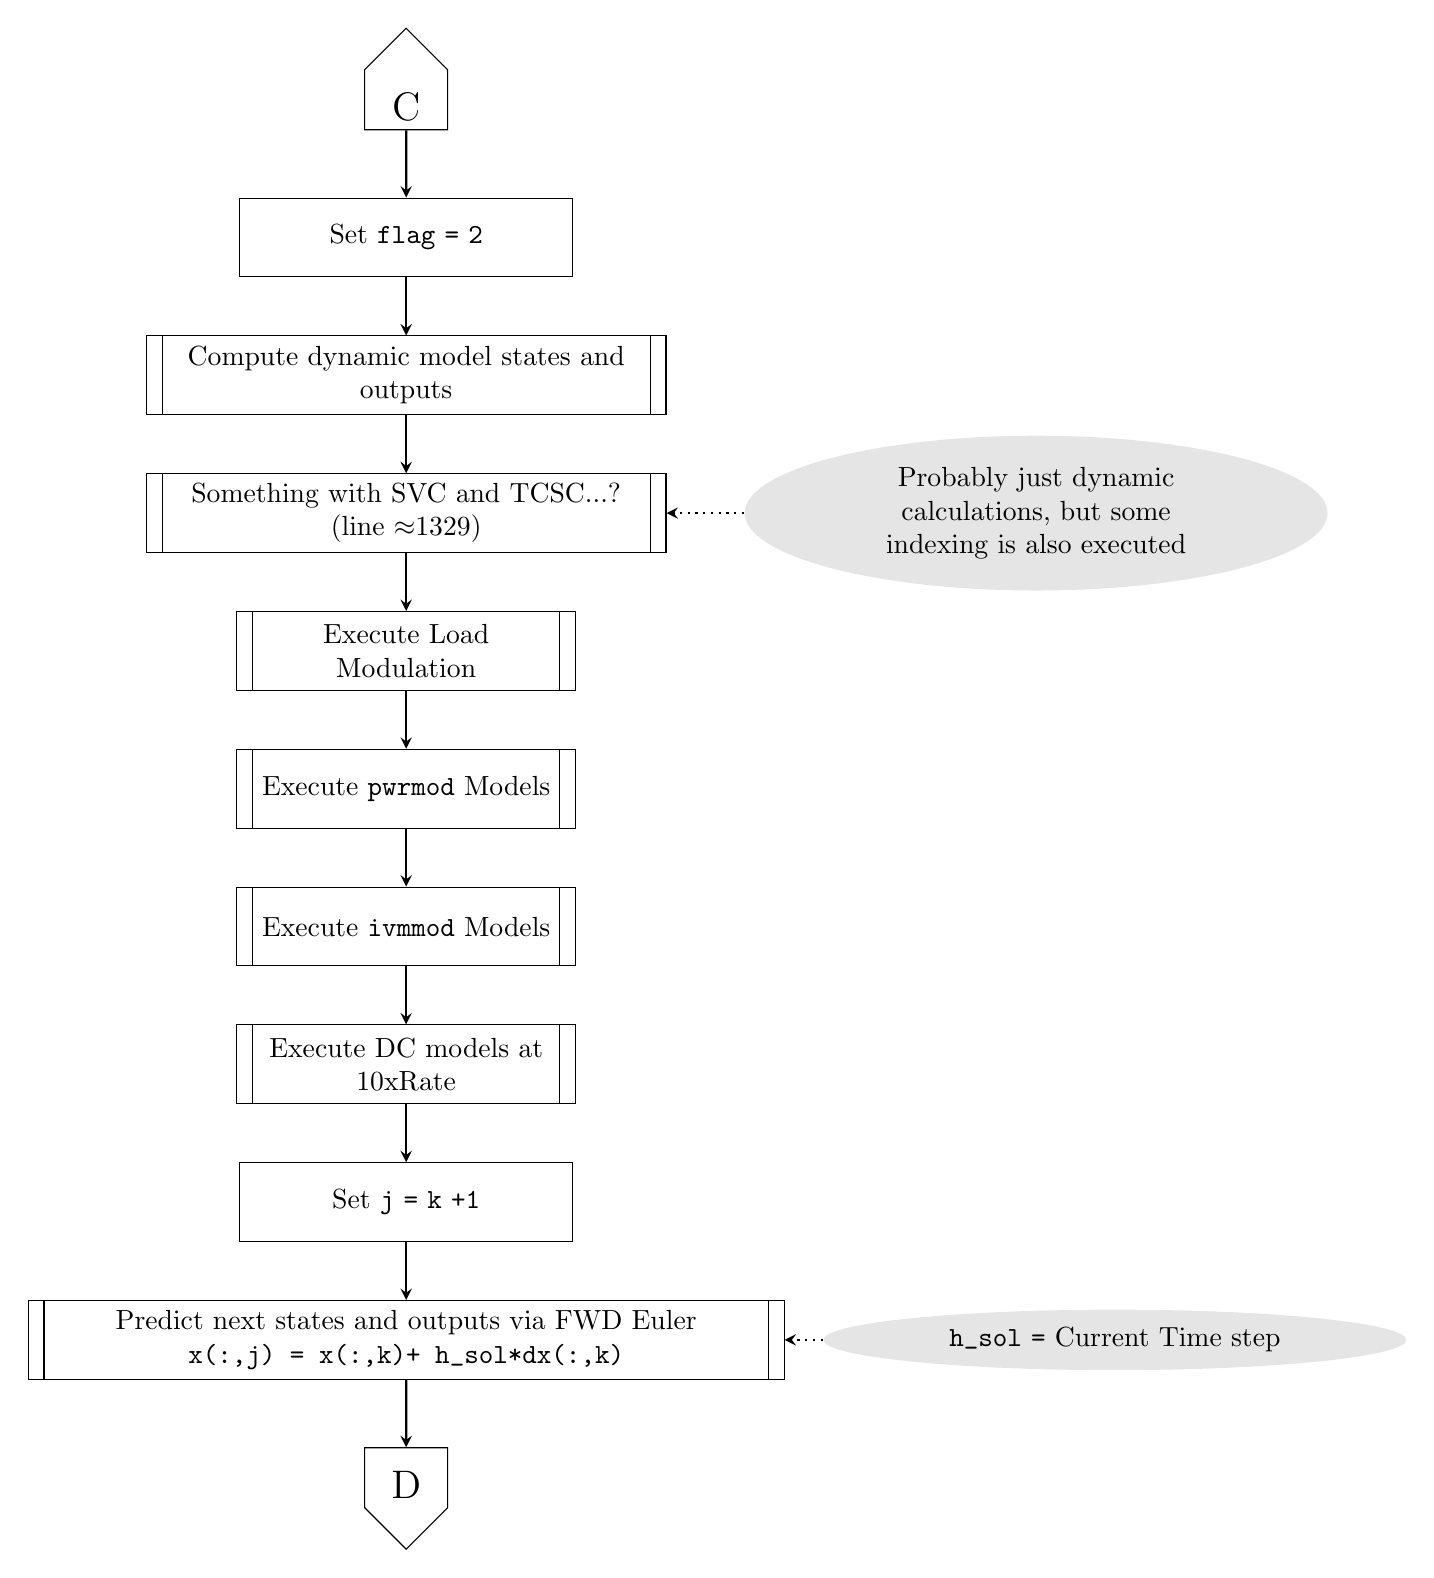
\begin{tikzpicture}[node distance=1.75cm] 
%----------------------------------------------------------------------------
% Placement of flowcart nodes
\node (page4Start) [pageconU] {\Large C};
\node (setFlagTWO1) [process, below of = page4Start] {Set \verb|flag = 2|};
\node (dynamics1) [subprocess, below of = setFlagTWO1, text width = 6 cm] {Compute dynamic model states and outputs};
\node (mystery1) [subprocess, below of = dynamics1, text width = 6 cm] {Something with SVC and TCSC...? (line $\approx$1329)};

\node (lmod1) [subprocess, below of = mystery1] {Execute Load Modulation};
\node (pwrmod1) [subprocess, below of = lmod1] {Execute \verb|pwrmod| Models};
\node (ivmmod1) [subprocess, below of = pwrmod1] {Execute \verb|ivmmod| Models};
\node (HVDCint1) [subprocess, below of = ivmmod1] {Execute DC models at 10xRate};

\node (setJ) [process, below of = HVDCint1] {Set \verb|j = k +1|};
\node (fwdEuler1) [subprocess, below of = setJ, text width = 9cm] {Predict next states and outputs via FWD Euler \verb|x(:,j) = x(:,k)+ h_sol*dx(:,k)|}; % unsure why math environment doesn't work...
\node (page4End) [pageconD, below of = fwdEuler1 ] {\Large D};

%----------------------------------------------------------------------------
% Lines
\draw [arrow] (page4Start) -- (setFlagTWO1);
\draw [arrow] (setFlagTWO1) -- (dynamics1);
\draw [arrow] (dynamics1) -- (mystery1);
\draw [arrow] (mystery1) -- (lmod1);

\draw [arrow] (lmod1) -- (pwrmod1);
\draw [arrow] (pwrmod1) -- (ivmmod1);
\draw [arrow] (ivmmod1) -- (HVDCint1);
\draw [arrow] (HVDCint1) -- (setJ);

\draw [arrow] (setJ) -- (fwdEuler1);
\draw [arrow] (fwdEuler1) -- (page4End);


%----------------------------------------------------------------------------
% Notes
\node [note, right of=fwdEuler1, node distance =9cm, text width = 5 cm ](note5){\verb|h_sol = |Current Time step}; % $\approx$Line 1468
\draw [arrow,dotted] (note5) -- (fwdEuler1);
\node [note, right of=mystery1, node distance =8cm, text width = 5 cm ](note6){Probably just dynamic calculations, but some indexing is also executed }; % $\approx$Line 1468
\draw [arrow,dotted] (note6) -- (mystery1);
\end{tikzpicture}
\pagebreak

%===============================================================================

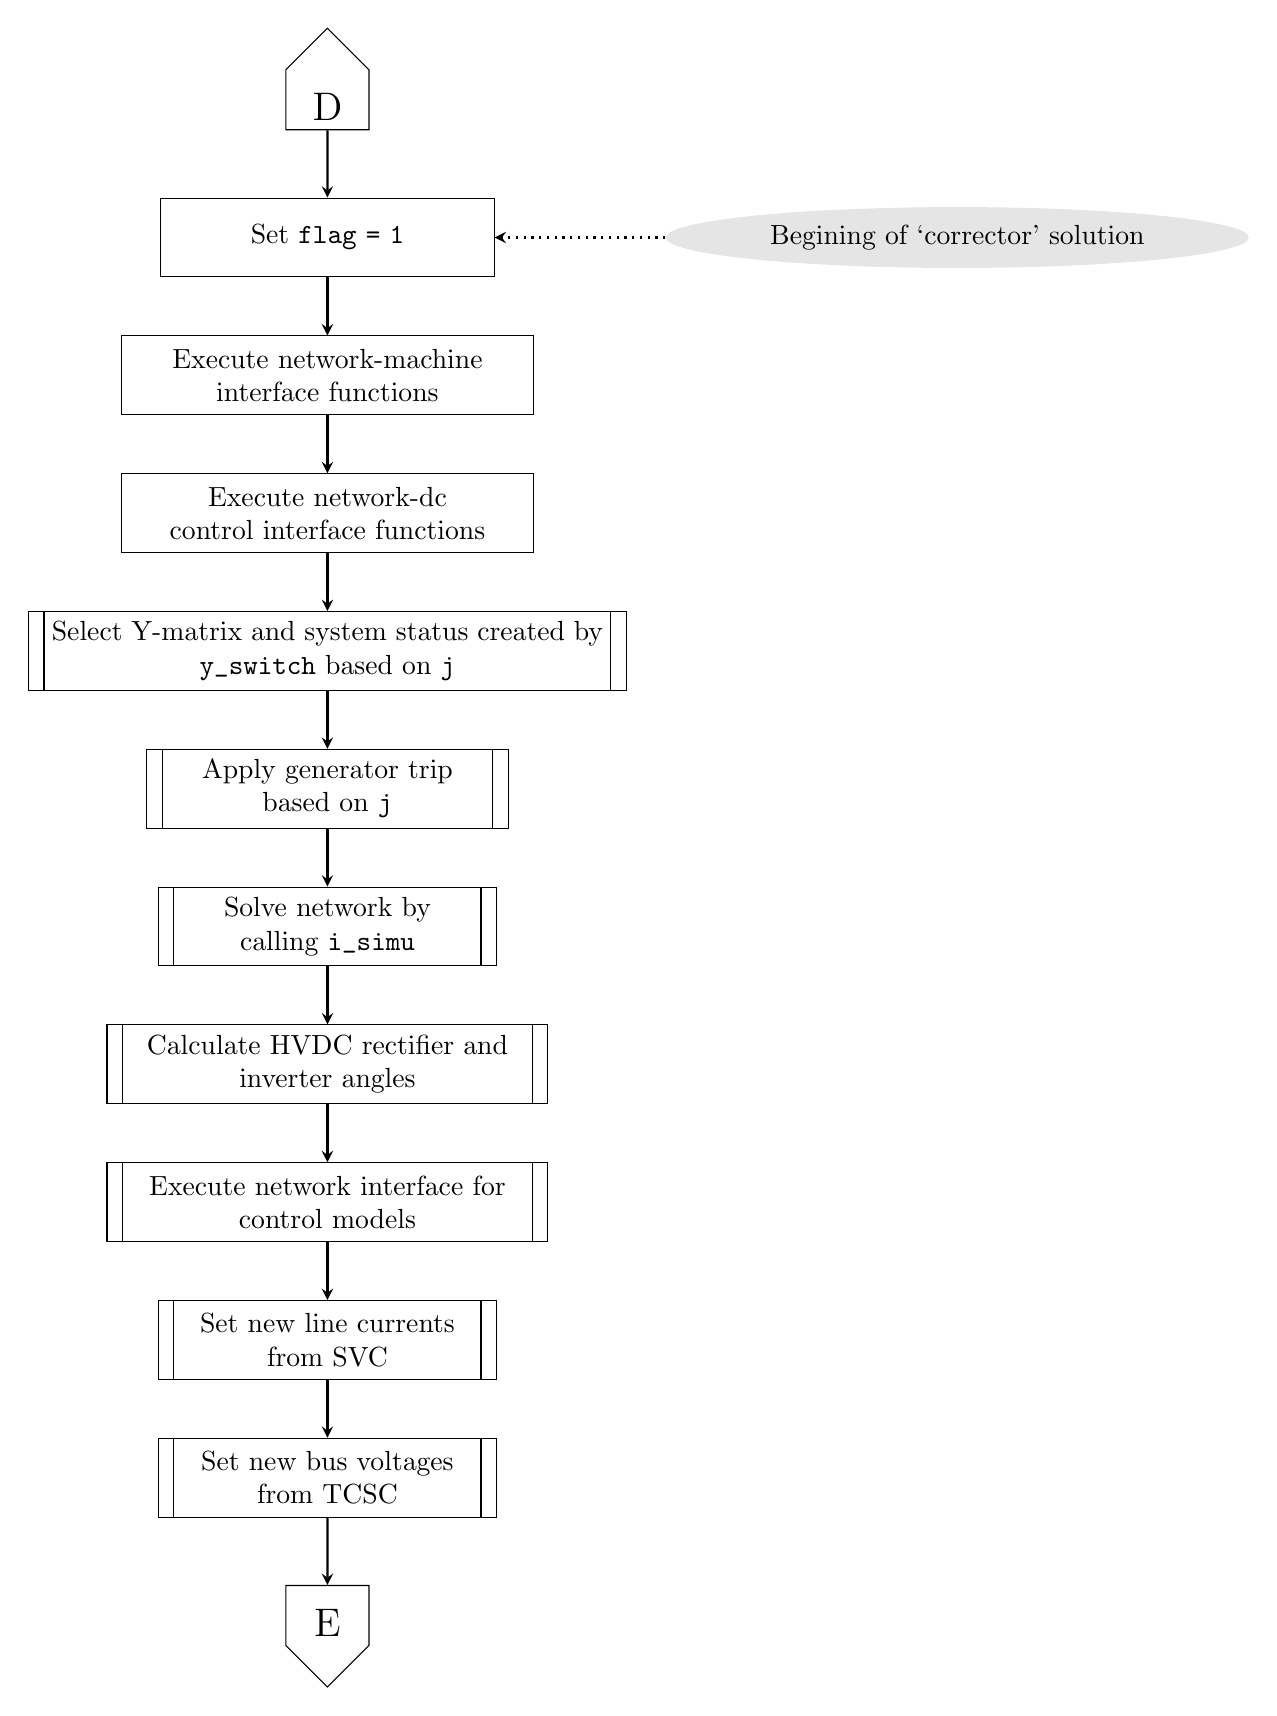
\begin{tikzpicture}[node distance=1.75cm] 
%----------------------------------------------------------------------------
% Placement of flowcart nodes
\node (page5Start) [pageconU ] {\Large D};

\node (setFlagONE2) [process, below of = page5Start] {Set \verb|flag = 1|};
\node (machineInterface2) [process, below of = setFlagONE2, text width = 5cm] {Execute network-machine interface functions};

\node (dcCTRLS2) [process, below of = machineInterface2, text width = 5cm] {Execute network-dc control interface functions};
\node (selectSYS2) [subprocess, below of = dcCTRLS2, text width = 7cm] {Select Y-matrix and system status created by \verb|y_switch| based on \verb|j|};
\node (applyGenTrip2) [subprocess, below of = selectSYS2, text width = 4cm] {Apply generator trip based on \verb|j|};
\node (solveNetwork2) [subprocess, below of = applyGenTrip2] {Solve network by calling \verb|i_simu|};

\node (HVDC2) [subprocess, below of = solveNetwork2, text width = 5 cm] {Calculate HVDC rectifier and inverter angles};
\node (ctrlNetwork2) [subprocess, below of = HVDC2, text width = 5 cm] {Execute network interface for control models};
\node (Isvc2) [subprocess, below of = ctrlNetwork2] {Set new line currents from SVC};
\node (Vtcsc2) [subprocess, below of = Isvc2] {Set new bus voltages from TCSC};
\node (page5End) [pageconD, below of = Vtcsc2 ] {\Large E};

%----------------------------------------------------------------------------
% Lines
\draw [arrow] (setFlagONE2) -- (machineInterface2);
\draw [arrow] (machineInterface2) -- (dcCTRLS2);

\draw [arrow] (dcCTRLS2) -- (selectSYS2);
\draw [arrow] (selectSYS2) -- (applyGenTrip2);
\draw [arrow] (applyGenTrip2) -- (solveNetwork2);
\draw [arrow] (solveNetwork2) -- (HVDC2);

\draw [arrow] (HVDC2) -- (ctrlNetwork2);
\draw [arrow] (ctrlNetwork2) -- (Isvc2);
\draw [arrow] (Isvc2) -- (Vtcsc2);

\draw [arrow] (page5Start) -- (setFlagONE2);
\draw [arrow] (Vtcsc2) -- (page5End);

%----------------------------------------------------------------------------
% Notes
\node [note, right of=setFlagONE2, node distance =8cm, text width = 5 cm ](note6){Begining of `corrector' solution}; % $\approx$Line 1468
\draw [arrow,dotted] (note6) -- (setFlagONE2);

\end{tikzpicture}
\pagebreak
%===============================================================================

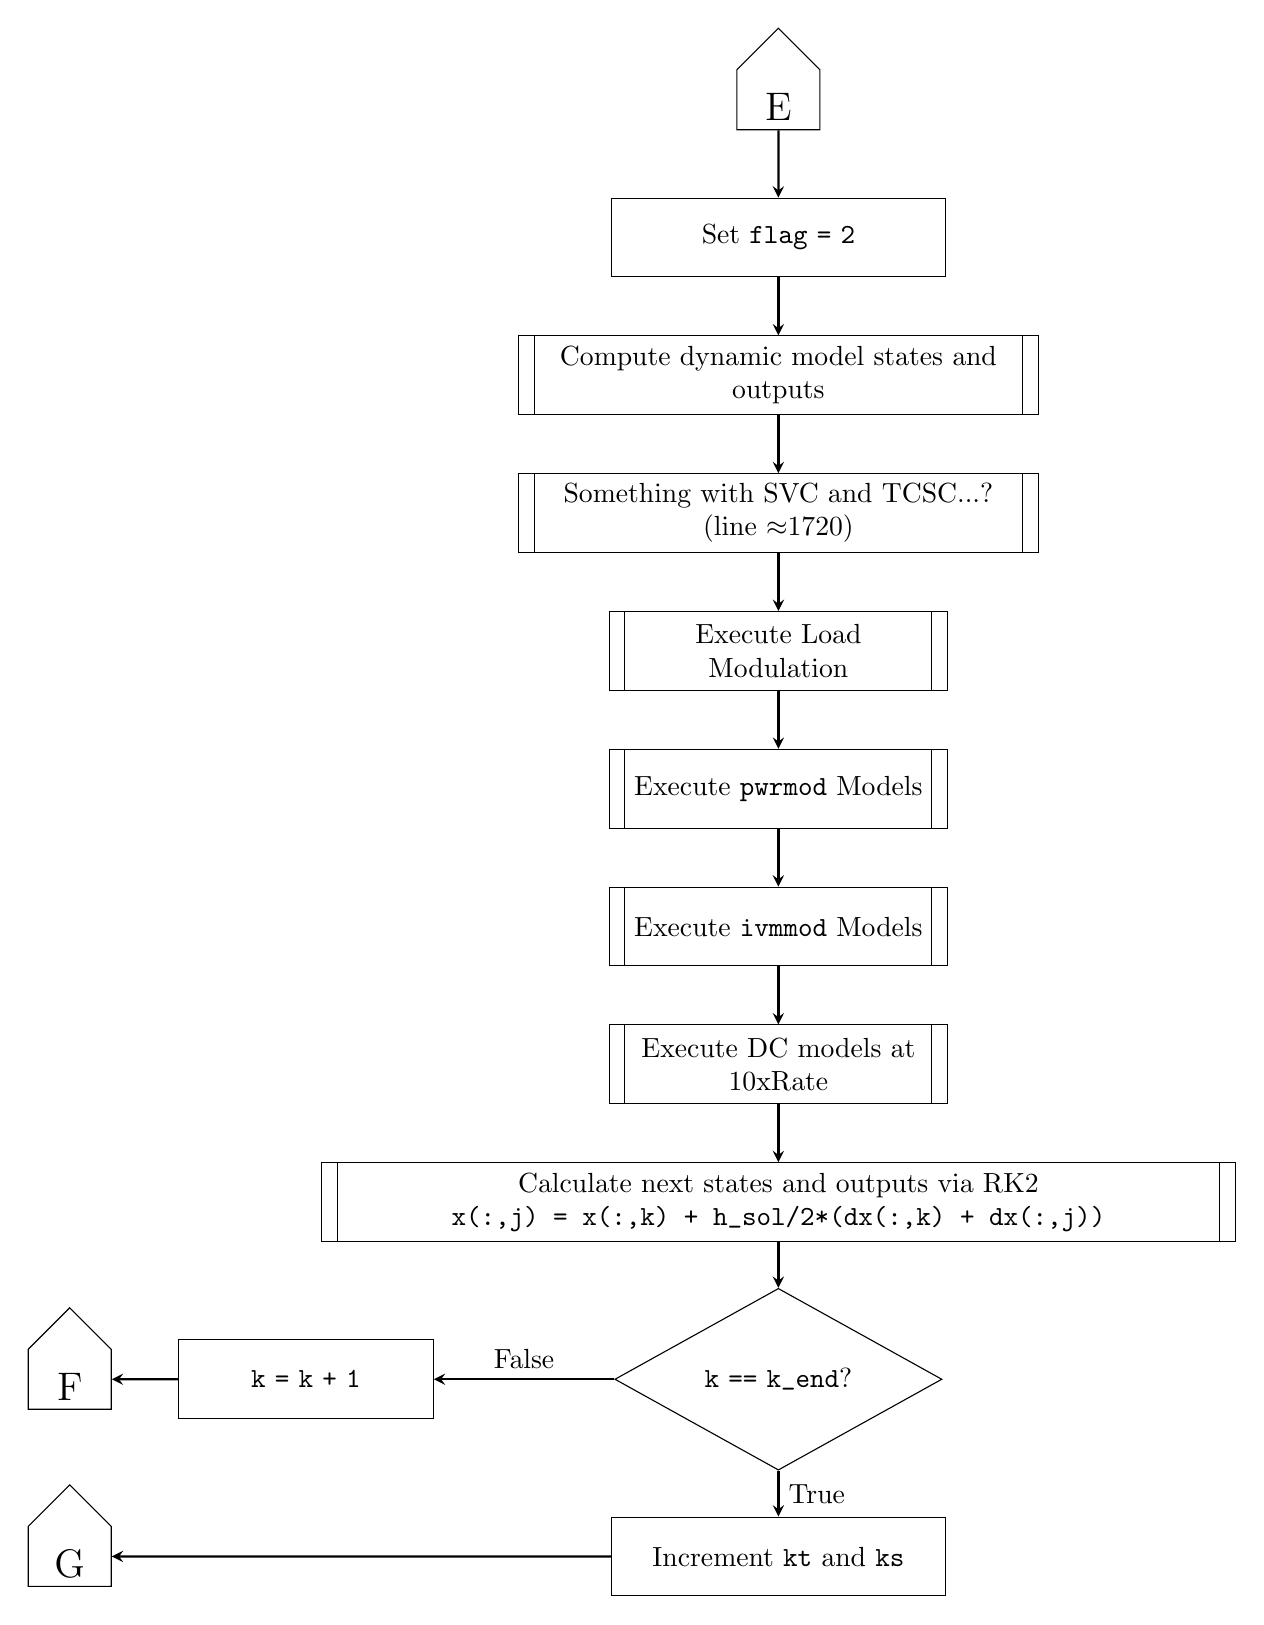
\begin{tikzpicture}[node distance=1.75cm] 
%----------------------------------------------------------------------------
% Placement of flowcart nodes
\node (page6Start) [pageconU ] {\Large E};

\node (setFlagTWO2) [process, below of = page6Start] {Set \verb|flag = 2|};
\node (dynamics2) [subprocess, below of = setFlagTWO2, text width = 6 cm] {Compute dynamic model states and outputs};
\node (mystery2) [subprocess, below of = dynamics2, text width = 6 cm] {Something with SVC and TCSC...? (line $\approx$1720)};

\node (lmod2) [subprocess, below of = mystery2] {Execute Load Modulation};
\node (pwrmod2) [subprocess, below of = lmod2] {Execute \verb|pwrmod| Models};
\node (ivmmod2) [subprocess, below of = pwrmod2] {Execute \verb|ivmmod| Models};
\node (HVDCint2) [subprocess, below of = ivmmod2] {Execute DC models at 10xRate};

\node (RK2) [subprocess, below of = HVDCint2, text width = 11cm] {Calculate next states and outputs via RK2 \verb|x(:,j) = x(:,k) + h_sol/2*(dx(:,k) + dx(:,j))|};
\node (forOver) [decision, below of=RK2, yshift=-.5cm, text width=3cm] {\verb|k == k_end|?};
\node (counterInc) [process, below of = forOver, yshift=-.5cm] {Increment \verb|kt| and \verb|ks|};

\node (incK) [process, left of = forOver, text width = 3 cm, node distance = 6 cm] {\verb|k = k + 1|};

%----------------------------------------------------------------------------
% Lines
\draw [arrow] (page6Start) -- (setFlagTWO2);
\draw [arrow] (setFlagTWO2) -- (dynamics2);
\draw [arrow] (dynamics2) -- (mystery2);
\draw [arrow] (mystery2) -- (lmod2);

\draw [arrow] (lmod2) -- (pwrmod2);
\draw [arrow] (pwrmod2) -- (ivmmod2);
\draw [arrow] (ivmmod2) -- (HVDCint2);
\draw [arrow] (HVDCint2) -- (RK2);

\draw [arrow] (RK2) -- (forOver);

%----------------------------------------------------------------------------
% Notes

%----------------------------------------------------------------------------
% Draw Decision Lines
\draw [arrow] (forOver) --  node[anchor=west] {True} (counterInc);
\draw [arrow] (forOver) -- node[anchor=south, midway] {False} (incK);

%----------------------------------------------------------------------------
% additional off page connects and lines
\node (continueFor) [pageconU, left of = incK, node distance = 3 cm ] {\Large F};
\node (endFor) [pageconU, left of = counterInc, node distance = 9 cm ] {\Large G};
\draw [arrow] (counterInc) -- (endFor);
\draw [arrow] (incK) -- (continueFor);
\end{tikzpicture}
\pagebreak
\begin{comment}

%===============================================================================
%===============================================================================

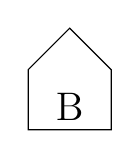
\begin{tikzpicture}[node distance=1.75cm] 
%----------------------------------------------------------------------------
% Placement of flowcart nodes
\node (page3Start) [pageconU ] {\Large B};


%----------------------------------------------------------------------------
% Lines


%----------------------------------------------------------------------------
% Notes


\end{tikzpicture}
\pagebreak
\end{comment}

\end{document}